\chapter{Performance and Analysis}
\renewcommand{\baselinestretch}{\mystretch}
\label{chap:Perf}
%\setlength{\parindent}{0pt}

\section{Platform comparison}

\fref{fig:raw-seq-p-c} clearly shows the relative performance figures of all testing platforms. The NP1380 platform is unable to meet the minimum requirement of 50 fps sequences, therefore most performance analysis for \texttt{VixenConsole} was done on the Raspberry Pi B+ platform.

\section{Implementation comparison}

\begin{figure*}[t]
  \centering
  \subfloat[Raspberry Pi B+]{\includegraphics[width=0.6\textwidth]{Figs/RPi-perf.eps}%
  \label{fig:perf_RPi}}
  \hfil
  \subfloat[Raspberry Pi 3B]{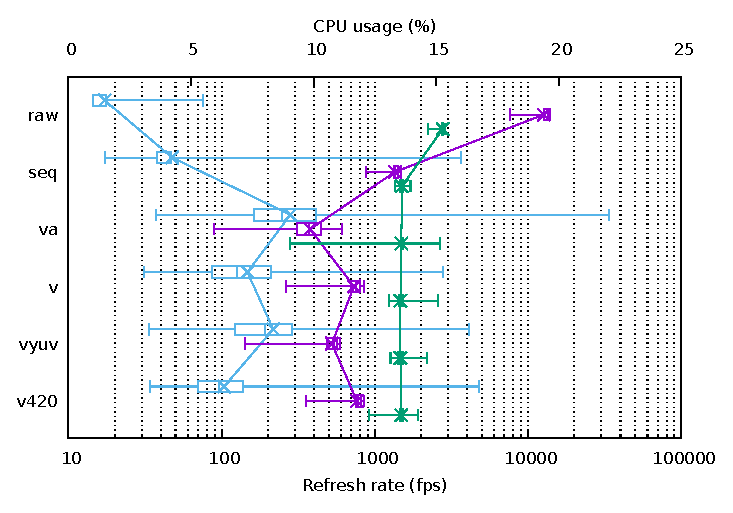
\includegraphics[width=0.6\textwidth]{Figs/RPi3-perf.eps}%
  \label{fig:perf_RPi3}}
  \hfil
  \subfloat[Jetson TX2]{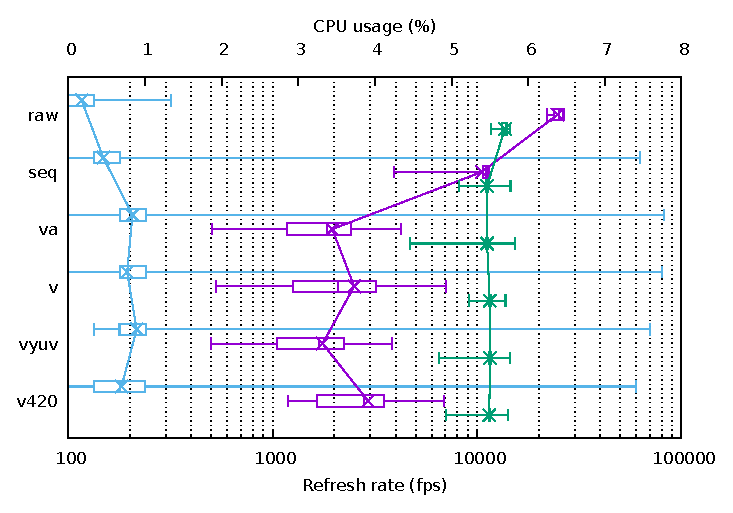
\includegraphics[width=0.6\textwidth]{Figs/TX2-perf.eps}%
  \label{fig:perf_TX2}}
  \caption{\footnotesize Performances of different implementations on different platforms}
  \label{fig:perf}
\end{figure*}

\fref{fig:perf_RPi} shows the performance comparison between different implementations on Raspberry Pi B+. \texttt{VixenLinky} (referenced by \texttt{raw}) has the highest refresh rate for its simplicity. \texttt{VixenConsole} with the ``Raw'' sequence format (referenced by \texttt{seq}) has the second highest performance. The unlimited playback performance drops to almost half when using a \texttt{rgb24} encoded video as the input (referenced by \texttt{v}). The performance drops again by a small factor when audio stream was also added to the video input (referenced by \texttt{va}). The video only playback performance of \texttt{yuv420p} encoding (referenced by \texttt{v420}) is only a little bit higher than the lossless \texttt{rgb24} encoding (\texttt{v}), whereas the performance of lossless \texttt{yuv444p} encoding (referenced by \texttt{vyuv}) is noticeably lower. Therefore, video encoding format of \texttt{libx264rgb} with \texttt{rgb24} pixel format is more suitable for encoding video sequences.

\ca{For other platforms, \fref{fig:perf_RPi3} and} \fref{fig:perf_TX2} shows the performance comparison on \ca{the Raspberry Pi 3B and} the NVIDIA Jetson TX2 platforms \ca{respectively}. \ca{The refresh rate easily reached a few hundreds of fps on the Raspberry Pi 3B platform, and more on the TX2 platform, which} has \ca{a} similar single core CPU performance to the Microsoft Windows laptop. \ca{On the TX2 platform, the} maximum refresh rates \ca{reached} over 1,000 fps for playback and 10,000 fps for controllers. For the 50 fps \ca{test} sequence, the CPU usage almost never reaches above $1 \%$. \ca{Compared} to the original Vixen application struggling to \ca{reach a} 50 fps refresh rate on Microsoft Windows, the new playback engine definitely achieved \ca{substantial} performance improvements.

\cmt{Test different container formats?}
